%*----------- SLIDE -------------------------------------------------------------
\begin{frame}[c]{A tropa dos quatro incríveis}
    %\transboxin[duration=1,direction=30]
    A simulação deverá ser desenvolvida com 4 unidades Darwin-OP, comumente esta unidade é utilizada para desafios em competições de robótica.
    \newline

    A tropa será composta por 4 Darwin-OP, e deverá realizar duas missões:
    \begin{itemize}
        \item marchar em forma unida em linha;
        \item realizar corrida de revezamento.
    \end{itemize}

    \begin{figure}
        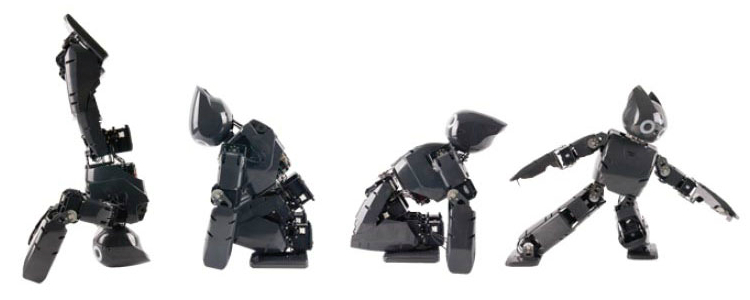
\includegraphics[trim = 0 20 0 50, clip, width=0.8\textwidth]{darwin-op-sequencia}
        %\caption{.}
    \end{figure}
%*----------- notes
    \note[item]{Notes can help you to remember important information. Turn on the notes option.}
\end{frame}
%-
%*----------- SLIDE -------------------------------------------------------------
\begin{frame}[t]{Algumas regras}
    \begin{itemize}
        \item A marcha deverá ser realizada diante de um percurso de 2 metros.
        \item A marcha e a corrida de revezamento deverão serem realizadas numa pista de corrida;
        \item A corrida deverá ser realizada numa pista de 8 metros;
        \item Cada Darwin-OP deverá percorrer 2 metros para realizar o revezamento;
        \item A região de revezamento deverá ser uma área de até 0.4 metros;
        \item O conceito para o revezamento será o de alinhar-se os dois Darwin-OP durante até 15 segundos a uma distância de no máximo 0.2 metros entre ambos, ou seja será considerado passagem de bastão quando os dois Darwin-OP passarem 15 segundos com movimentos sincronizados a uma distância máxima de 0.2 metros dentro da região de revezamento;
        \item A pista de corrida deverá ser considerada analogamente a uma pista real;
        \item A lateral da pista deverá ter lados de 2 metros;
        \item Considerar sempre os critérios de uma corrida de revezamento.
    \end{itemize}
   
    % \begin{columns}[t]
    %     \column{.45\textwidth}
    %         detalhar sistemas em subconjuntos\\
    %         listar possíveis modos de falhas\\
    %         analisar cada modo de falha, juntamente com suas possíveis causas e sintomas
    %     \column{.45\textwidth}
    %         estimar os efeitos de cada modo de falhas\\
    %         estimar a criticidade de cada efeito\\
    %         identificar ações para minimizar falhas
    % \end{columns}
%*----------- notes
    \note[item]{Notes can help you to remember important information. Turn on the notes option.}
\end{frame}
%-
%*----------- SLIDE -------------------------------------------------------------
\begin{frame}[c]{A pista}
    \begin{figure}
        %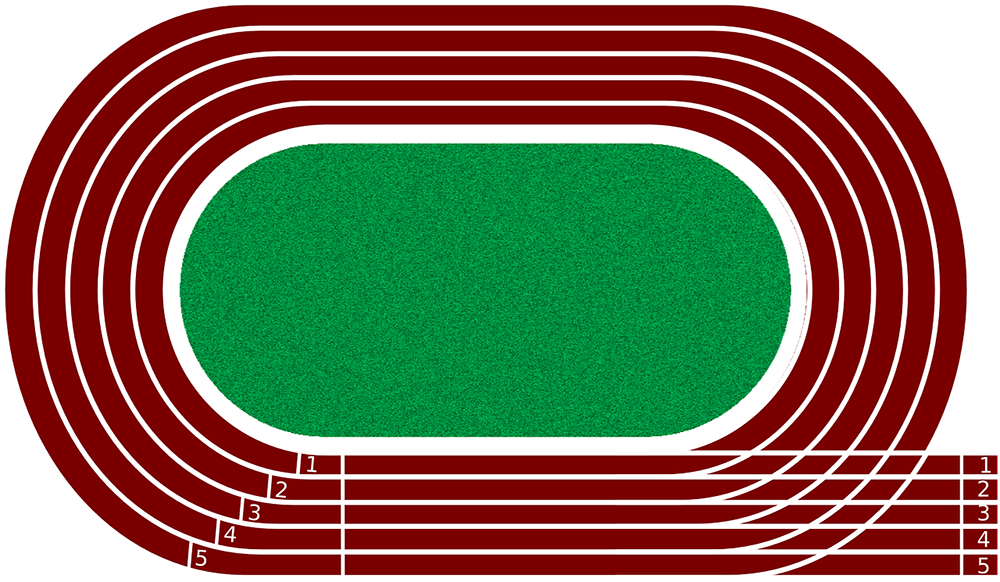
\includegraphics[width=0.7\textwidth]{pista_corrida}
       
        \roundpic[xshift=0cm,yshift=0cm]{3cm}{7cm}{pista_corrida}
          
        \caption{Formato de um pista de corrida.\cite{agostini2007}}
    \end{figure}
%*----------- notes
    \note[item]{Notes can help you to remember important information. Turn on the notes option.}
\end{frame}
%-